One of the core debates of economic theory is that of the rationality of agents. Keynesian economics was the dominant school of thought until the 1970s which saw the rise of New Classical economics\autocite{Hartley2013}. Lucas and Sargent were two key spearheads of this movement with their influential paper titled "After Keynesian Macroeconomics", key to their complaints were the lack of microeconomic foundations in Keynesian models\autocite{Lucas1979}. Real business cycle theory, a major branch of New Classical economics believed that business cycles were a rational response to exogenous shocks to the economy and were perfectly efficient. However, this also meant that business cycles would not arise endogenously as firms and consumers would learn over time the behavior of the economy as they, as a whole, acted rationally. Though Keynesianism has since gained in popularity after the 2007 financial crisis, these lessons of New Classical Economics continue to influence the microfoundations of macroeconomic New Keynesian models.

Wegener, et al. directly based their inventory cycle model on that developed by Metzler. However, both of these models required that firms be boundedly rational which, to a New Classical economist, would be an unrealistic assumption not rooted in microeconomic foundations. However, it is appropriate to limit the ability for firms to predict the future if the reason for it can be appropriately explained. Behavioral economics and experimental data has frequently shown a gap between perfectly rational, utilitarian behavior and what is actually practiced by humans\autocite{Smith2006}; however, we would expect firms to behave more rationally than individuals. Some models make use of stochastic shocks in order to drive dynamic behavior; these tend to follow a New Classical real business cycle framework as these stochastic processes are the primary drivers of economic cycles. Another possible process is that of chaotic behavior. Under these conditions, it is possible for the economy to reside in a completely deterministic state while still making it impossible for firms to accurately predict future states in the economy . Having the unpredictability of the economy be primarily driven by chaotic processes rather than stochastic ones is of great use from a policy perspective due to the nature of having parameters to influence rather than random behavior, this is discussed in greater detail by Faggini and Parziale\autocite{Faggini2012}. 

The growth model described in Chapter \ref{ch:metzlerian-expanded} has a basis in Metzler's inventory cycle but also incorporates a multiplier-accelerator mechanism for endogenous investment and consumption and the results of numerical simulations of the model display the possibility of chaos, in addition to other phenomena such as the existence of multiple attractors. Of particular note is the bifurcation diagram and Lyapunov exponent plot of the parameter $s$. The marginal propensity to save, under the initial conditions and other parameter choice tested, do not display any stable fixed points. In fact, over the possible range of $s$, most possible trajectories are chaotic; one such trajectory is displayed in Figure \ref{growth_chaotic-timeseries}.
\begin{figure}
    \centering
    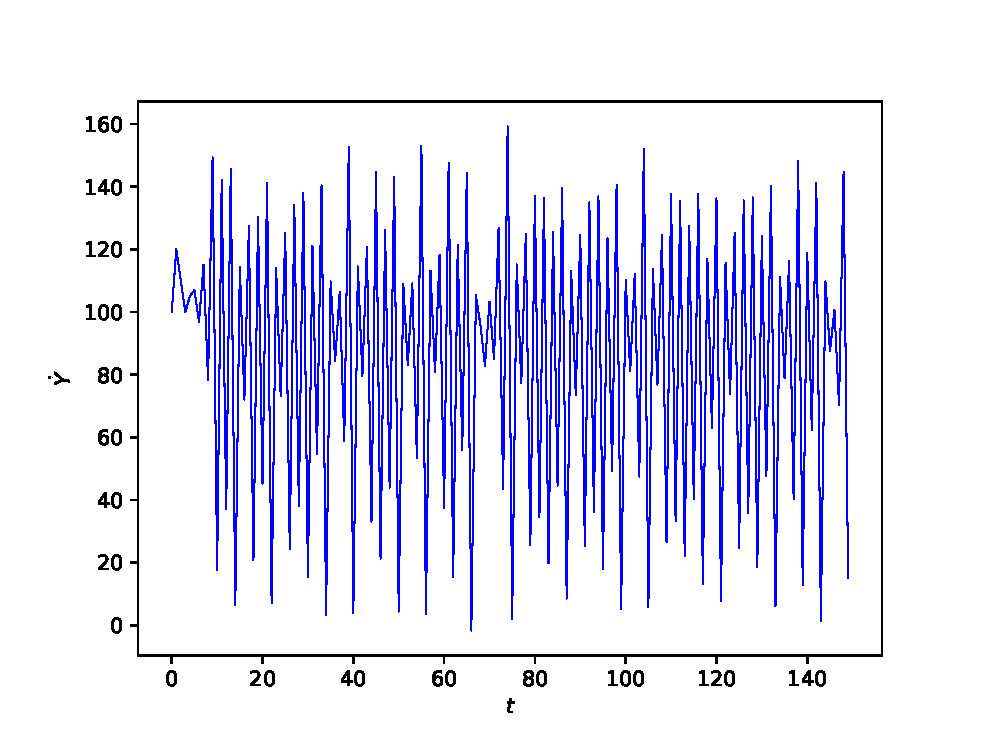
\includegraphics[height=0.4\textheight]{./metzlerian_growth/chaotic_timeseries.eps}
    \caption{Timeseries plot of income growth rate over 150 iterations. $s=0.4,\ k=0.3,\ v=500,\ q=0.001$. Initial values of $\dot Y$ are: 100, 120, 110, 100, 105, 107}
    \label{growth_chaotic-timeseries}
\end{figure}
Figure \ref{metzlerian_growth-kLyapunov} also displays chaotic behavior; however, this only occurs when $k$ is very large and is unlikely to occur in a real scenario. Both $s$ and $k$ are the two parameter choices that describe the behavior of the agents of the economy in non-monetary terms. Based on the results of Figure \ref{metzlerian_growth-kLyapunov} and \ref{metzlerian_growth-kbifurcation}, variation of this parameter has minor effects on the growth rate of the economy compared to variation of $s$. This implies that the choice of inventory proportion, outside of the extreme cases, has a minor impact on the long-run dynamics of the model. This is not to say that the inventory cycle is itself a minor factor of the economy; removal of the inventory cycle changes this model to an unsimplified version of the model presented in Chapter \ref{ch:multiplier-accelerator}. This model features a functionally identical mechanism for consumption with a Robertson lag and although the form of the function for endogenous investment differs between the two models, they are qualitatively similar for the reasons mentioned in Chapter \ref{ch:metzlerian-expanded}.

\begin{figure}
    \centering
    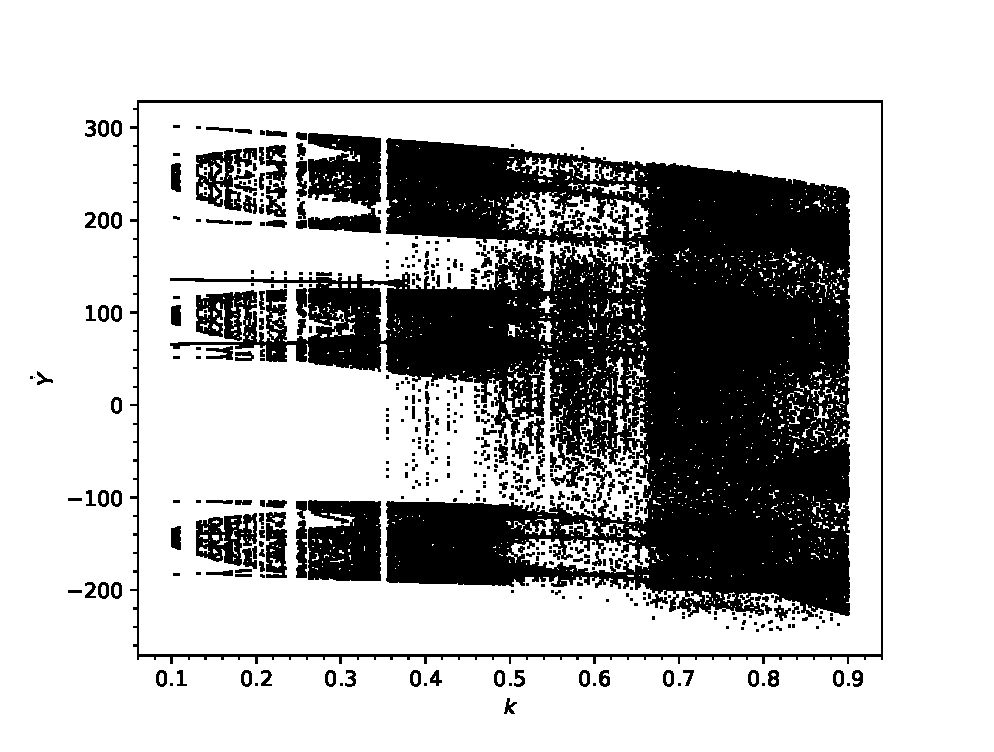
\includegraphics[height=0.4\textheight]{./metzlerian_growth/kbifurcation2.eps}
    \caption{Bifurcation diagram varying $k$ between 0.1 and 0.9. Initial conditions and other parameters are held constant as described in Figure 4.1 except $s=0.7$}
    \label{metzlerian_growth-kbifurcation2}
\end{figure}
\begin{figure}
    \centering
    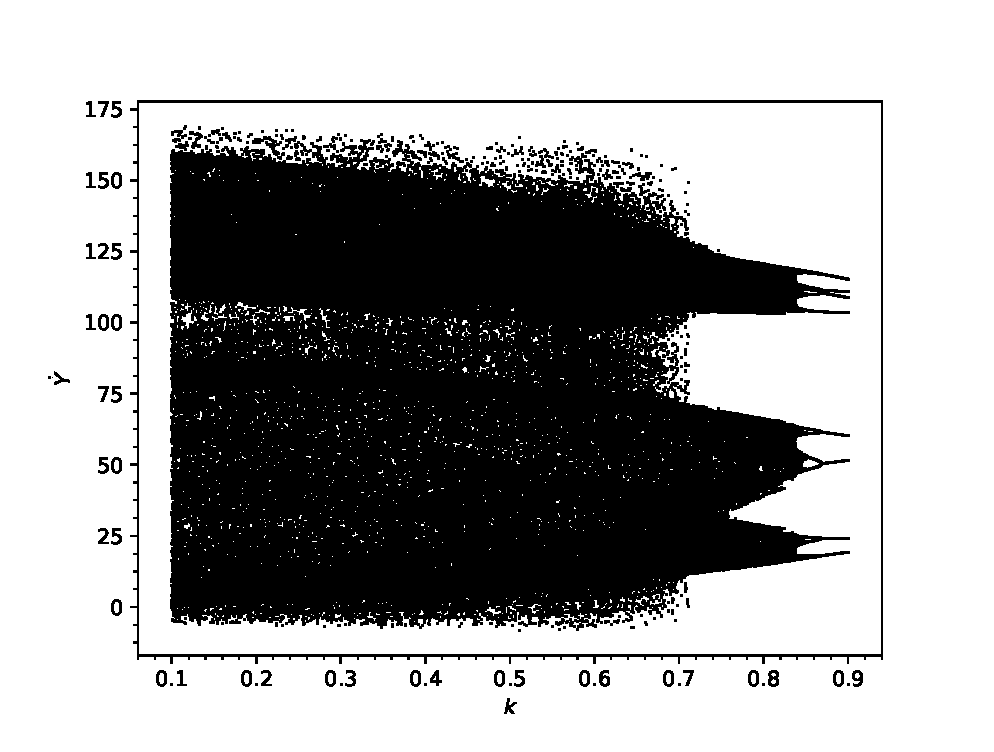
\includegraphics[height=0.4\textheight]{./metzlerian_growth/kbifurcation3.eps}
    \caption{Bifurcation diagram varying $k$ between 0.1 and 0.9. Initial conditions and other parameters are held constant as described in Figure 4.1 except $s=0.3$}
    \label{metzlerian_growth-kbifurcation3}
\end{figure}
Figure \ref{metzlerian_growth-kbifurcation2} and \ref{metzlerian_growth-kbifurcation3} displays behavior that is qualitatively distinct from that in Figure \ref{metzlerian_growth-kbifurcation} despite both plots showing the long-run behavior of the model with the same variation in $k$. However, by increasing or decreasing $s$ until it is in the chaotic regime presented in Figure \ref{metzlerian_growth-sLyapunov}, we see that varying $k$ can have a significant effect on the long-run dynamics of growth at even more reasonable values of $k$.

$q$ determines the maximum and minimum of the investment function and $v$ is the primary determinant of of the FWHM of the function. Given the initial conditions, we see chaotic behavior when large quantities of investment are allowed by the investment curve, i.e. $q$ is small. The initial growth values vary between 100 and 120 so it appears that allowing investment to exceed growth in quantity results in instability;  however, there do still remain windows of order in the primary chaotic region of $q$. Interestingly, the system appears to be relatively ordered for most values of $v$; however, there is a small region where $250<v<750$ that displays chaotic behavior in Figure \ref{metzlerian_growth-vLyapunov}. Figure \ref{metzlerian_growth-chaotic_timeseries2} displays one such trajectory, of note is how the model cycles between both positive and negative growth regimes but also between high amplitude variation and low amplitude variation. It appears that under this parametrization, high absolute values of income change reduce investment; however, instead of ending in stability, this lower income variance state drives higher levels of investment shifting the model back to a high income variance regime.
\begin{figure}
    \centering
    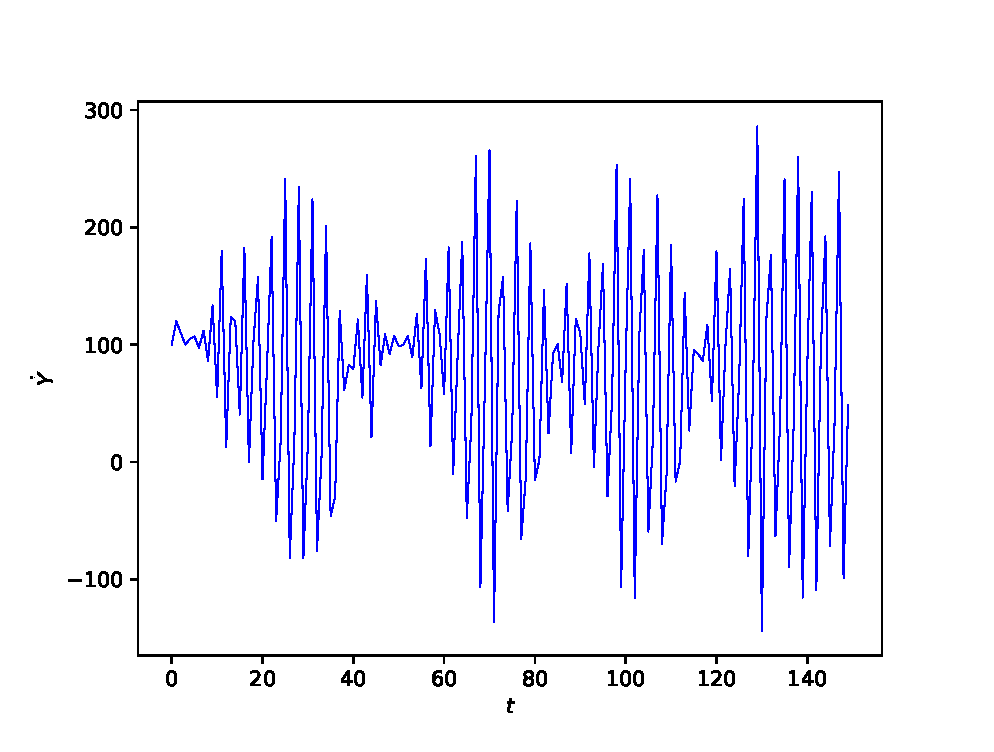
\includegraphics[height=0.4\textheight]{./metzlerian_growth/chaotic_timeseries2.eps}
    \caption{Timeseries plot of income growth rate over 150 iterations. $s=0.6,\ k=0.3,\ v=416,\ q=0.001$}
    \label{metzlerian_growth-chaotic_timeseries2}
\end{figure}

$v$ and $q$ are likely to change depending on the state of the economy, the government's fiscal policy, and the technology available. The investment curve bends back and has a "width" due to the presumption of changes in public investment and taxes in response to the state of the economy and the presence of other limiting factors in income growth. If the government decides to loosen their concern to output variation, the width of the investment curve would increase. The height of the function can change over time as the required level of investment needed to sustain an output level changes can change with improvements in technology or human capital. 

Generally speaking, larger values of early initial growth compared to the later values of initial growth results in a lower overall long-run growth. This can be seen in Figure \ref{metzlerian_growth-y0bifurcation}, \ref{metzlerian_growth-y1bifurcation}, and \ref{metzlerian_growth-y2bifurcation}. The relationship is reversed if growth is larger for more recent time periods as can be seen in Figure \ref{metzlerian_growth-y3bifurcation}, \ref{metzlerian_growth-y4bifurcation}, and \ref{metzlerian_growth-y5bifurcation}. Ignoring the chaotic behavior, this model implies that relatively sharp drops in growth rate result in lower growth horizons whereas large spikes in growth rate result in high growth horizons. The non-linear nature of the model and presence of multiple attractors complicates this idea although the trend is still present. This economy is susceptible to external forces; an exogenous but temporary increase in the growth rate will result in a long-run increase in growth rate. The economy is thus able to use aid in order to accelerate its own growth. Likewise, if an external shock reduces output relative to its usual behavior, this can result in a decreased growth rate in the long-run. 

The goal of this model was to incorporate both a Robertson and Lundberg lag and endogenize investment change. This was done in order to provide a mechanism to explain why firms on aggregate are unable to accurately predict future consumption. Many models use stochastic processes in order to rationalize this; however, this model shows the presence of chaotic behavior. Under a chaotic regime, firms would only be able to predict future behavior by knowing the exact state of the economy in the past; however, this is practically impossible as even small differences between the actual initial conditions and estimated initial conditions will result in very different future results by the definition of chaos. 

Much work remains to be done on this model in order to better describe the quantity and structure of the multiple attractors and an explanation of the model's response to changing parameters. As more work is done on the mathematics of higher-order non-linear iterated maps, it may become possible to analytically solve for the behavior of the model although this remains unlikely for the near future. More work also needs to be done to differentiate between quasi-periodic behavior and chaotic behavior in the model, although both are inherently unpredictable, quasi-periodic behavior provides a more consistent structure to long-run behavior while still preventing firms from accurately determining future outcomes.

This model could also be expanded upon in a variety of ways. This economy is closed; however, most modern economies are open to foreign trade to varying degrees. This provides another income channel as well as providing another outlet for investment that does not improve the domestic economy. A more complex investment mechanism could also be incorporated, by explicitly separating public and private investments and removing the x-axis symmetry seen in the current curve. There are many possible ways for firms to predict future consumption, a simple average was used here although a conditional expectation that would allow firms to better use past information and learn from their previous experiences would help alleviate concerns regarding rational behavior by the firms. This however can lead to mathematical complications if firms have infinite possible memory. These additions could improve the realism of the model while still using chaos as the primary driver of chaotic behavior. 



